\documentclass{beamer}
\usepackage[pantone315]{wwustyle}
\usepackage[ngerman]{babel}
\usepackage[utf8]{inputenc}
\usepackage{lmodern}

% \usepackage[style=verbose, backend=biber]{biblatex}
%\addbibresource{res/literatur.bib}
%\setbeamertemplate{bibliography item}{\insertbiblabel}

\usepackage{graphicx}
\graphicspath{{res/}{img/}{../img/}}
\usepackage{amsmath}
\usepackage{amssymb}
\usepackage{siunitx}

% Section-Ueberschrift Slides
\AtBeginSection[]{
  \begin{frame}
  \vfill
  \centering
  \begin{beamercolorbox}[sep=8pt,center,shadow=true,rounded=true]{title}
    \usebeamerfont{title}\insertsectionhead\par%
  \end{beamercolorbox}
  \vfill
  \end{frame}
}


\title[short title]{Title} %TODO add title
\subtitle{Subtitle} %TODO add subtitle
\institutelogo{}
\institutelogosmall{}
\author{Autor 1, Autor 2, Autor 3} %TODO add author
\date{01.01.1970} %TODO add date

\begin{document}

% Title
\begin{frame}[plain]
\maketitle
\end{frame}



\begin{frame}
\frametitle{Übersicht}

% Inhaltsverzeichnis
\tableofcontents

\end{frame}


\section{Motivation}

\begin{frame}
\frametitle{Motivation}
\begin{center}
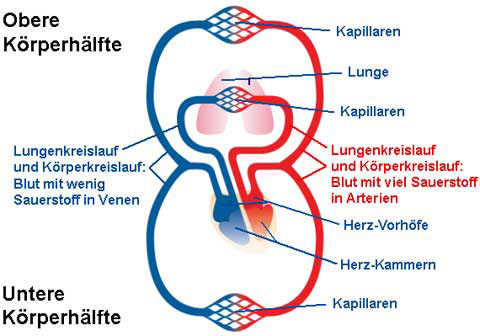
\includegraphics[scale=0.55]{motivation.jpg}  
\end{center}
\end{frame}

\section{Herleitung des 0D-Modells}

\begin{frame}
\frametitle{Herleitung}

\end{frame}

\section{Das 0D-Modell}

\begin{frame}
\frametitle{0D-Modell}
\begin{equation}
  \begin{aligned}
    C \frac{dP_1}{dt} &= Q_1 - Q_2\\
    L \frac{dQ_2}{dt} &= P_1 - P_2 - RQ_2
  \end{aligned}
\end{equation}
\pause
Analog zu elektrischen Bauteilen:
\begin{center}
  \includegraphics[width=0.6\textwidth]{kirchhoff.png}
\end{center}
\end{frame}

\begin{frame}
\frametitle{0D-Modell}
  \begin{center}
  	\begin{tabular}[!htb]{c c c}
  		Hydraulisch	&	Variable	&	Elektrisch\\
  		\hline
  		Druck	&	$P$	&	Spannung\\
  		Flussrate	&	$Q$	&	Stromstärke\\
  		Blut-Viskosität	&	$R$	&	Widerstand\\
  		Blut-Trägheit	&	$L$	&	Induktivität\\
  		Ader-Elastizität	&	$C$	&	Kapazität
  	\end{tabular}
  \end{center}

\end{frame}

\section{Simulation}

\begin{frame}
\frametitle{Simulation}
\begin{columns}
  \begin{column}{0.45\textwidth}
    \begin{itemize}
      \item Numerische Lösung\\
      \item Python/\texttt{scipy}
      \item grobe Parameterwahl:\\
      {$P_{1/2}, Q_{1/2}, R, L, C = 1$}
    \end{itemize}
  \end{column}
  \begin{column}{0.55\textwidth}
    \begin{center}
      \centering
      \includegraphics[width=1.1\textwidth]{simulation1.pdf}\\
    \end{center}
  \end{column}
\end{columns}


\end{frame}

\section{Fazit}

\begin{frame}
\frametitle{Fazit}

\end{frame}


% Print bibliography
% \begin{frame}[t,allowframebreaks]
% \frametitle{Sources}
% 	\printbibliography
% \end{frame}

\end{document}
